%!TEX root=../main.tex	% Optional

\section{JavaEE}

Die \textbf{Java Platform Enterprise Edition} enthält Spezifikationen welche die Java SE (\textbf{Java Standard Edition}) erweitert.

Diese Spezifikationen sind beispielsweise Funktionen wie \textit{Distributed Computing} und \textit{Web Services}.

Eine Java EE Application wird auf Application Server oder Microservices ausgeführt.

Siehe: \cite{wiki:javaee}

\clearpage

\section{Application Server}

Als Runtime für die \textbf{JavaEE Web Application} verwenden wir den \textit{Application Server} \textbf{Glassfish} \cite{github:glassfish}.

Der \textbf{Glassfish} Application Server soll in einem Docker Container gestartet werden, hierzu verwende ich das Dockerfile von Oracle \cite{github:oracle-docker-images}.

\begin{code}{sh}
    git clone https://github.com/oracle/docker-images/
    cd docker-images/GlassFish/5.0
    docker build -t glassfish5 .  # Container Builden
    docker run -d -p 4848:4848 -p 8080:8080 -p 8181:8181 -p 9009:9009 glassfish5  # Container starten
    xdg-open http://127.0.0.1:4848/  # Website starten
\end{code}

\clearpage

Der standard Benutzername ist \texttt{admin}, das Passwort ist \texttt{admin}.

Die Glassfish Startseite sieht folgendermaßen aus:

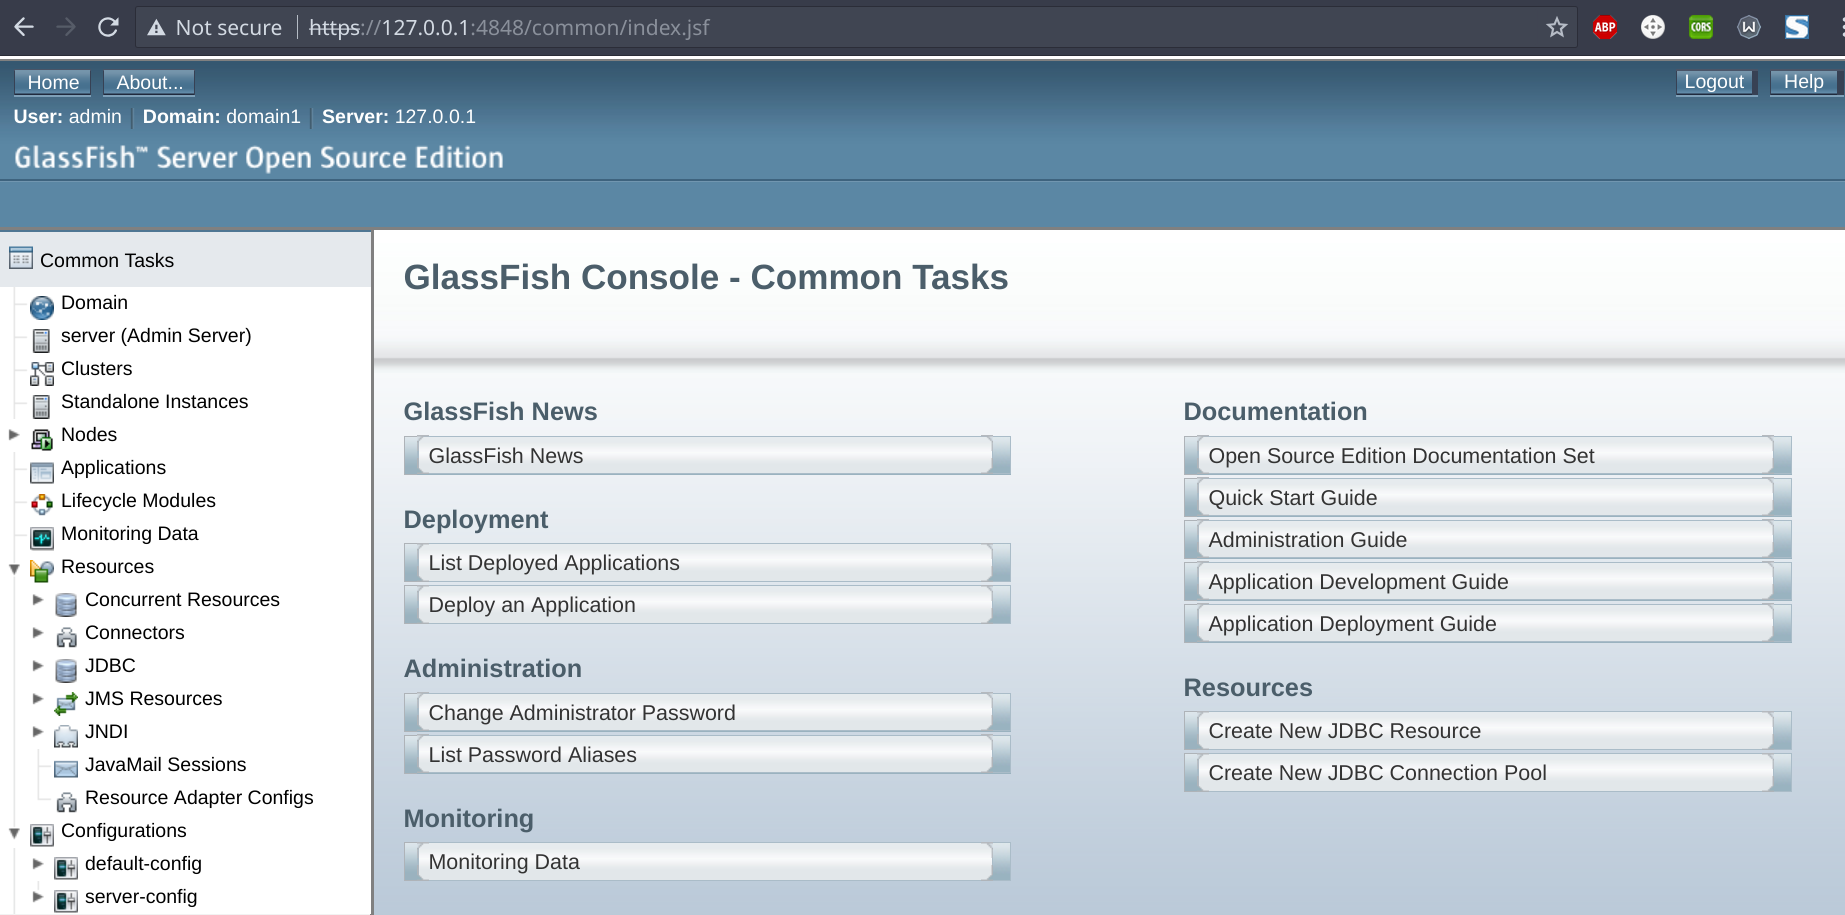
\includegraphics[width=\textwidth]{images/glassfish-home}

\clearpage

\section{Deploy}

Nun können wir eine JavaEE Applikation auf den Application Server deployen. Diese läuft dann unter der Glassfish JavaEE runtime welche zusätzliche Sicherheitsmaßnahmen und sonstige benötigte Features vorweist.

\begin{code}{sh}
    git clone https://github.com/javaee/tutorial-examples
    cd tutorial-examples
    mvn package
    cd web/jsf/ajaxguessnumber
\end{code}

Wir werden die Web Application \textbf{Ajax Guess Number} deployen.

Hierzu verwenden wir das Maven WAR Plugin in der \texttt{pom.xml} file:

\begin{code}{xml}
    <plugin>
        <artifactId>maven-war-plugin</artifactId>
        <configuration>
            <attachClasses>true</attachClasses>
            <webXml>target/web.xml</webXml>
            <webResources>
                <resource>
                    <directory>src/main/webapp</directory>
                    <filtering>true</filtering>
                </resource>
            </webResources>
        </configuration>
    </plugin>
\end{code}

Beim kompilieren wird nun auch ein \texttt{.war} (Web Archive/Web Application Resource) file erstellt, welche nun auf den Glassfish Server deployed wird.

Der Menüpunkt \textit{Deploy an Application} leitet auf folgende Seite weiter:

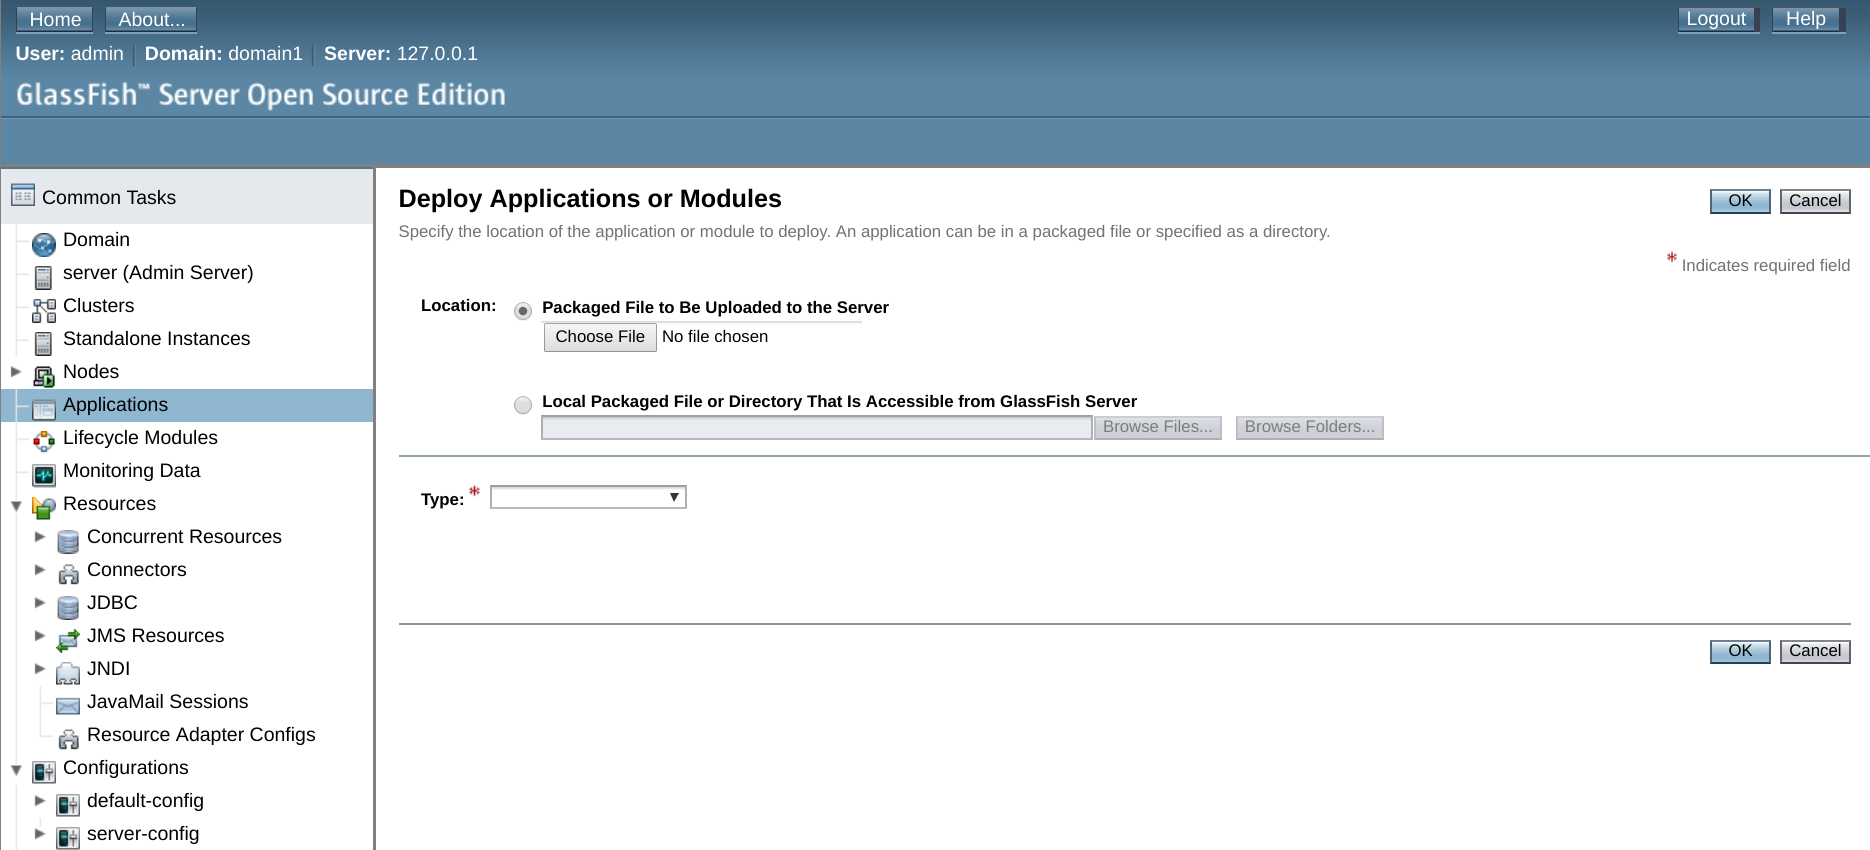
\includegraphics[width=\textwidth]{images/glassfish-deploy}

Das \texttt{war} Package muss ausgewählt und hochgeladen werden, und der Typ muss auf \textit{Web Application} gesetzt sein. Nun wird die Application im \textbf{Glassfish Application Pool} laufen.

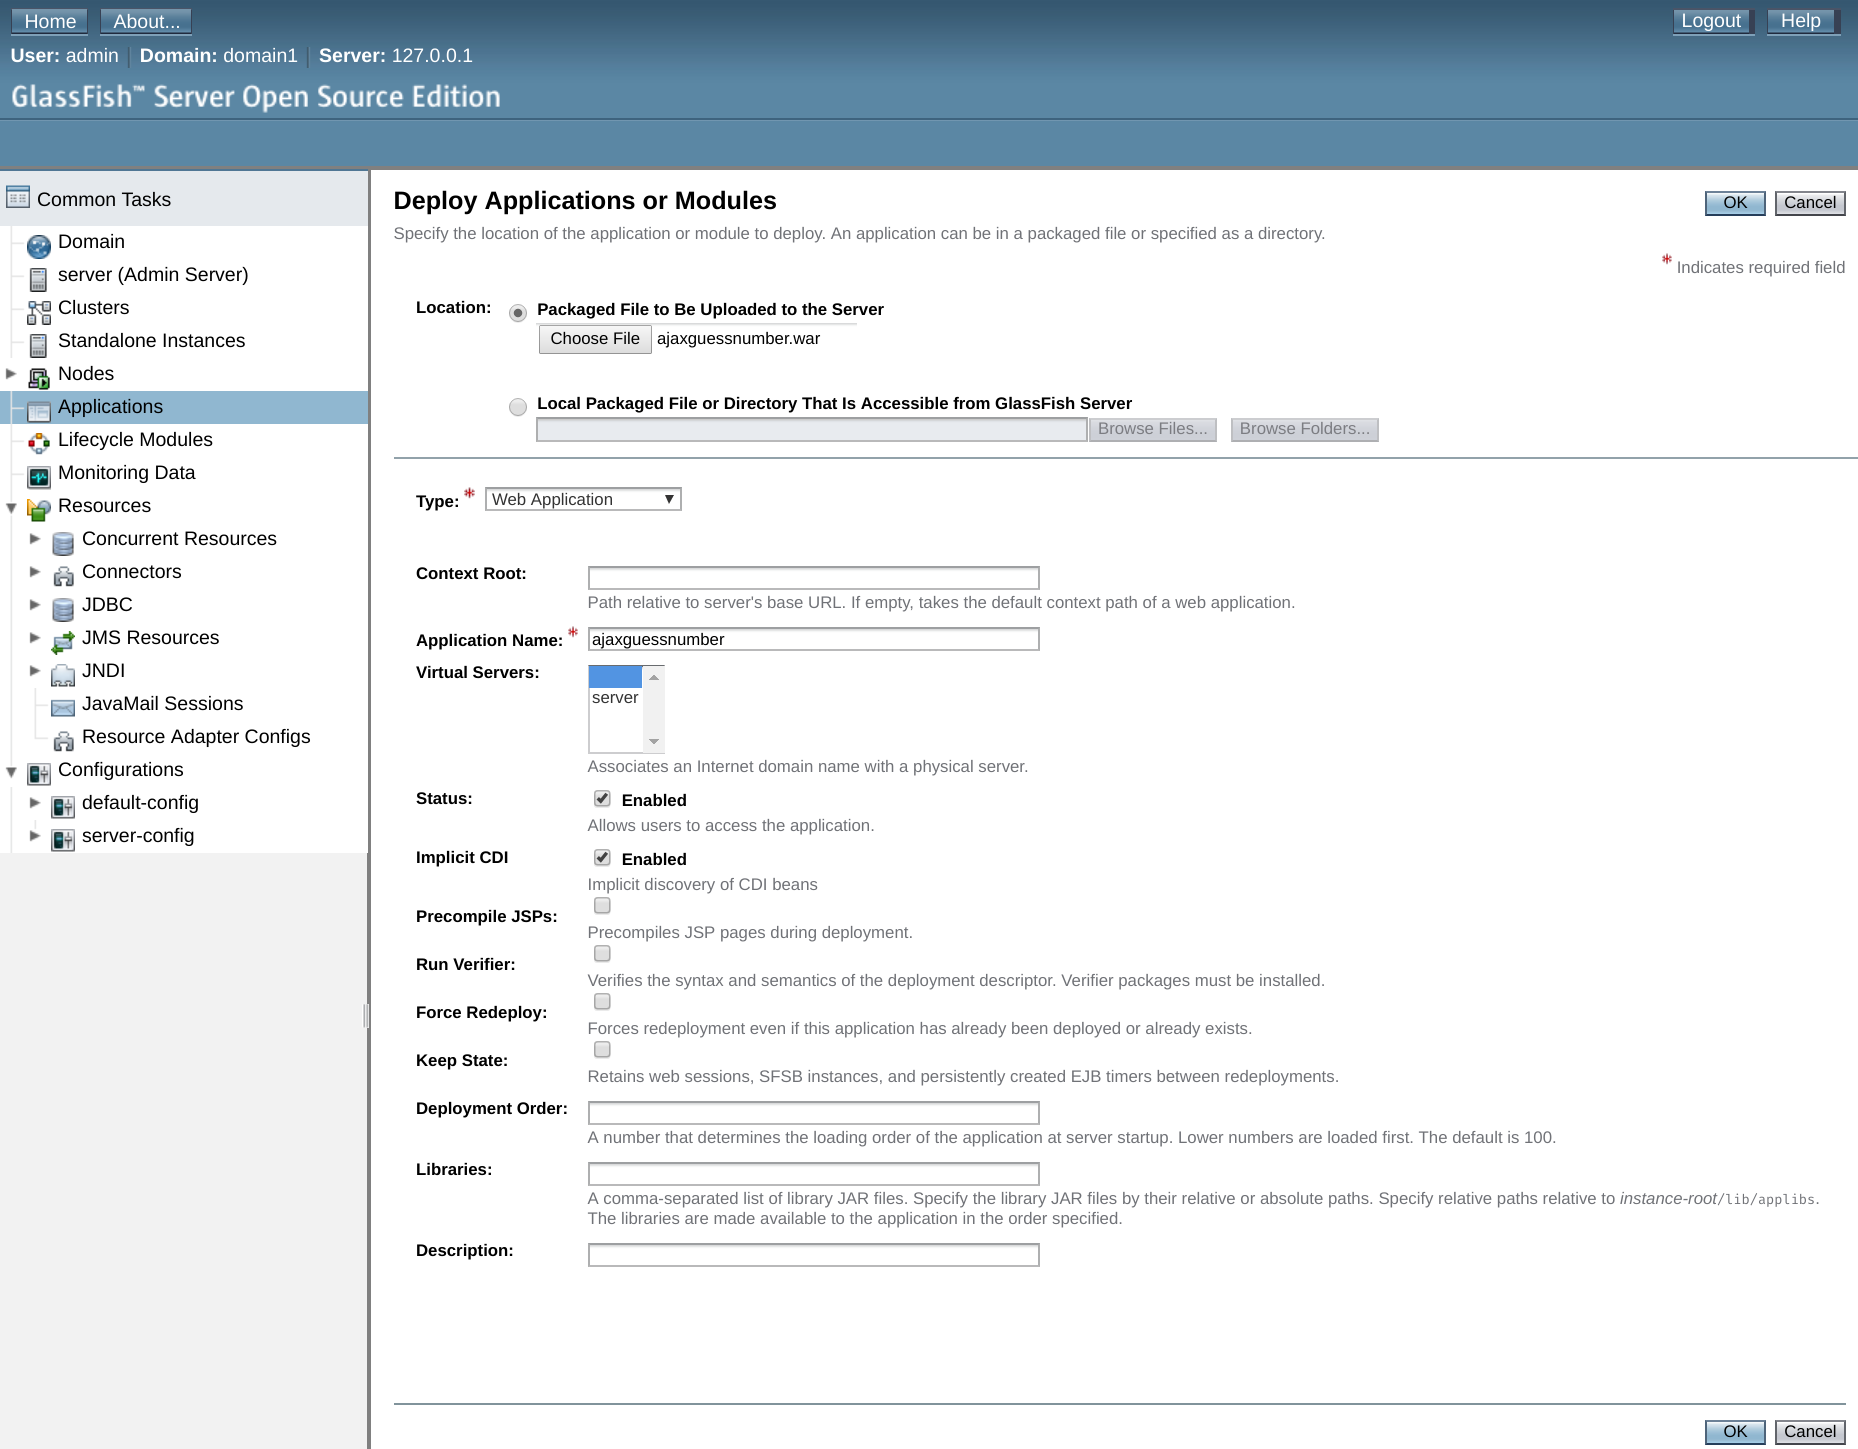
\includegraphics[width=\textwidth]{images/glassfish-deploy-war}

\clearpage

Alle Applications sind einsehbar unter dem Menüpunkt \textit{List Deployed Applications}, wo sie auch gestartet, erneut deployed und erneut geladen werden können.

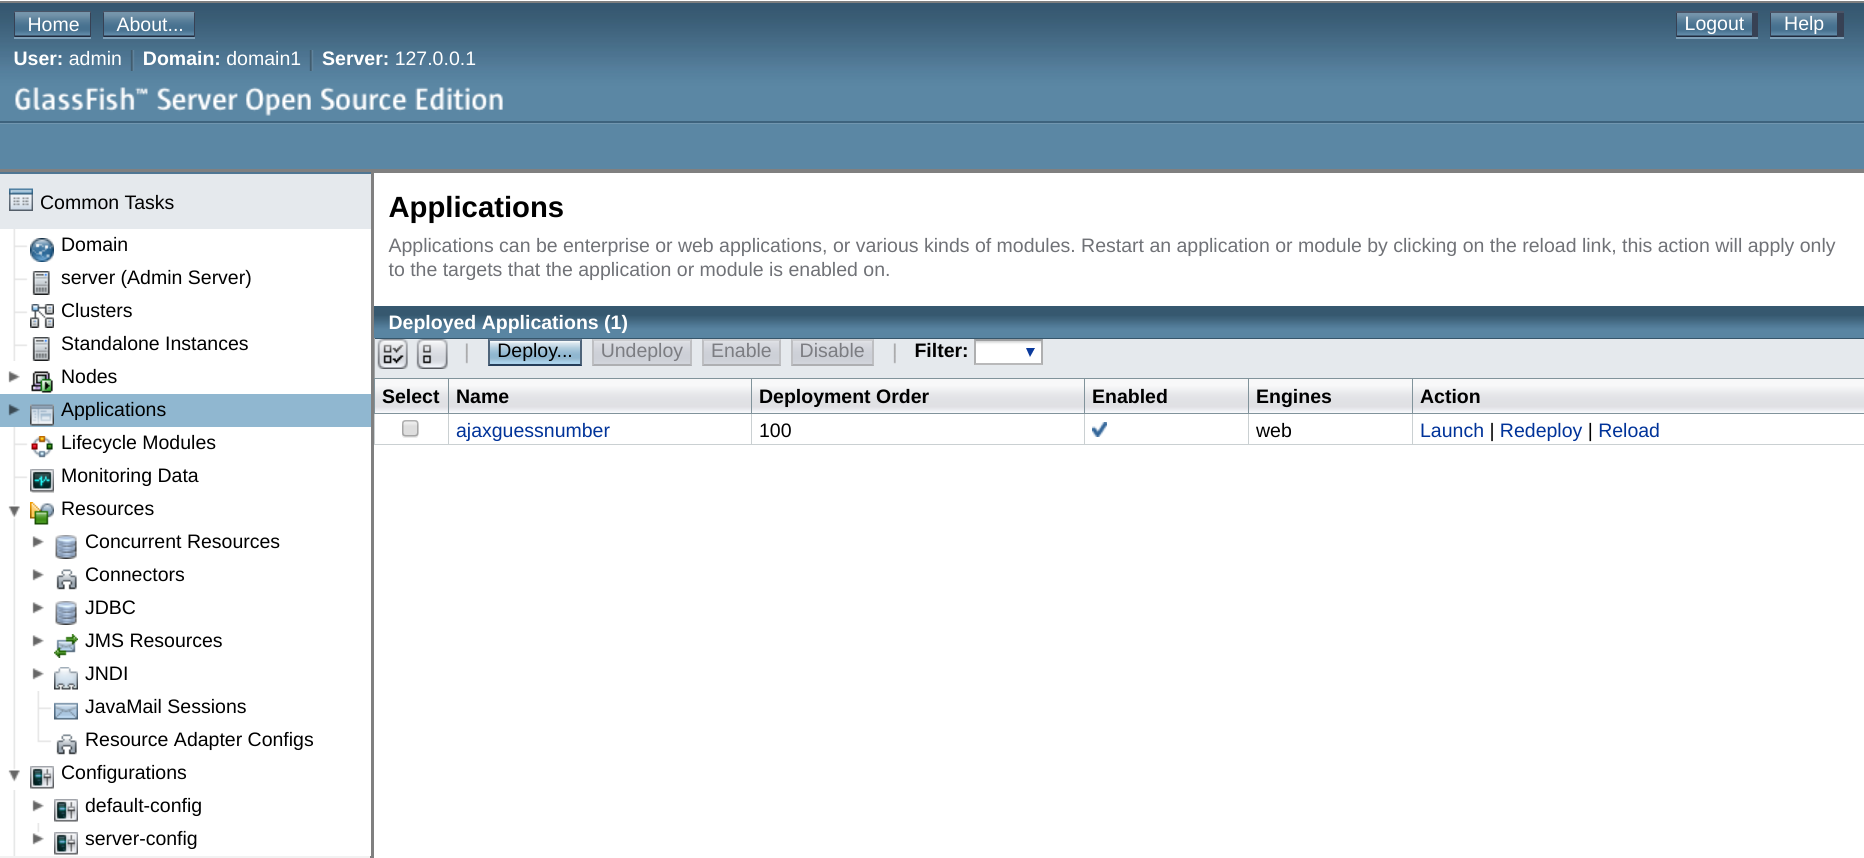
\includegraphics[width=\textwidth]{images/glassfish-apps}

Außerdem können unter \textit{Monitoring Data} -> \textit{View Log Files} jegliche logs eingesehen werden.
